\documentclass[aspectratio=169]{beamer}
\usetheme{Madrid}
\usecolortheme{default}

\usepackage[utf8]{inputenc}
\usepackage[T1]{fontenc}
\usepackage{booktabs}
\usepackage{amsmath}
\usepackage{graphicx}
\usepackage{siunitx}

\setbeamertemplate{navigation symbols}{}

\title{Fair and Transparent Human--AI Collaboration}
\subtitle{Personalized Exercise Recommendation with Knowledge Tracing}
\author{Joel Gedeon}
\date{AIMS 2026 Final Project}

\begin{document}

% Slide 1
\begin{frame}
  \titlepage
\end{frame}

% Slide 2
\begin{frame}{Task and Importance}
\small
\textbf{Goal:} Identify student proficiency on the target skill (needs support or not), then choose the best workflow action:
\begin{itemize}
  \item \textbf{A:} AI judges fit/not-fit autonomously
  \item \textbf{B:} Escalate fit/not-fit judgment to human teacher
  \item \textbf{C:} Request a short diagnostic quiz
\end{itemize}

\vspace{0.2cm}
\textbf{Decision objective}
\[
\pi^\*(x_t)=\arg\min_{a\in\{A,B,C\}} \mathbb{E}[\ell_t(a)\mid x_t] + c(a),
\]
where \(\ell_t(a)\) is action-dependent educational loss.

\vspace{0.2cm}
\textbf{Why this matters}
\begin{itemize}
  \item Wrong recommendations slow student learning progress.
  \item Teacher time is expensive and limited at scale.
  \item Unconstrained routing can create subgroup disparities.
\end{itemize}
\end{frame}

% Slide 3
\begin{frame}{Simulation and Policy Setup}
\small
\textbf{Input features (KT model):}
\begin{itemize}
  \item rolling student-skill correctness \(h_t\)
  \item attempt count \(a_t\)
  \item recency \(r_t=\log(1+\Delta_t)\)
  \item one-hot skill identity
\end{itemize}

\textbf{Calibration and uncertainty:}
\[
p_t=\sigma(\alpha z_t + \beta),\quad
q_t=\max(p_t,1-p_t),\quad
u_t=1-q_t.
\]

\textbf{Teacher simulation:}
\[
p_h(t)=\mathrm{clip}(0.88+\delta_g(g_t)+\delta_s(s_t)+\varepsilon_t,\ 0.60,\ 0.98),
\]
with \(\delta_g(1)=-0.18,\ \delta_g(0)=+0.05,\ \varepsilon_t\sim\mathcal{N}(0,0.03^2)\).

\textbf{Loss and action costs:}
\[
c(A)=0.0,\quad c(B)=0.9,\quad c(C)=0.5,\quad
\ell_t=
\begin{cases}
1-y_t,& \text{if judged fit}\\
0.4,& \text{if judged not fit}
\end{cases}
\]
\end{frame}

% Slide 4
\begin{frame}{Baseline vs Proposed Workflow}
\begin{center}
\IfFileExists{images/proposed_vs_baseline_flowchart.png}{
  \includegraphics[width=0.94\linewidth]{images/proposed_vs_baseline_flowchart.png}
}{
  \IfFileExists{../images/proposed_vs_baseline_flowchart.png}{
    \includegraphics[width=0.94\linewidth]{../images/proposed_vs_baseline_flowchart.png}
  }{
    \IfFileExists{images/proposed_vs_baseline_flowchart.txt.png}{
      
\includegraphics[width=0.94\linewidth]{images/proposed_vs_baseline_flowchart.txt.png}
    }{
      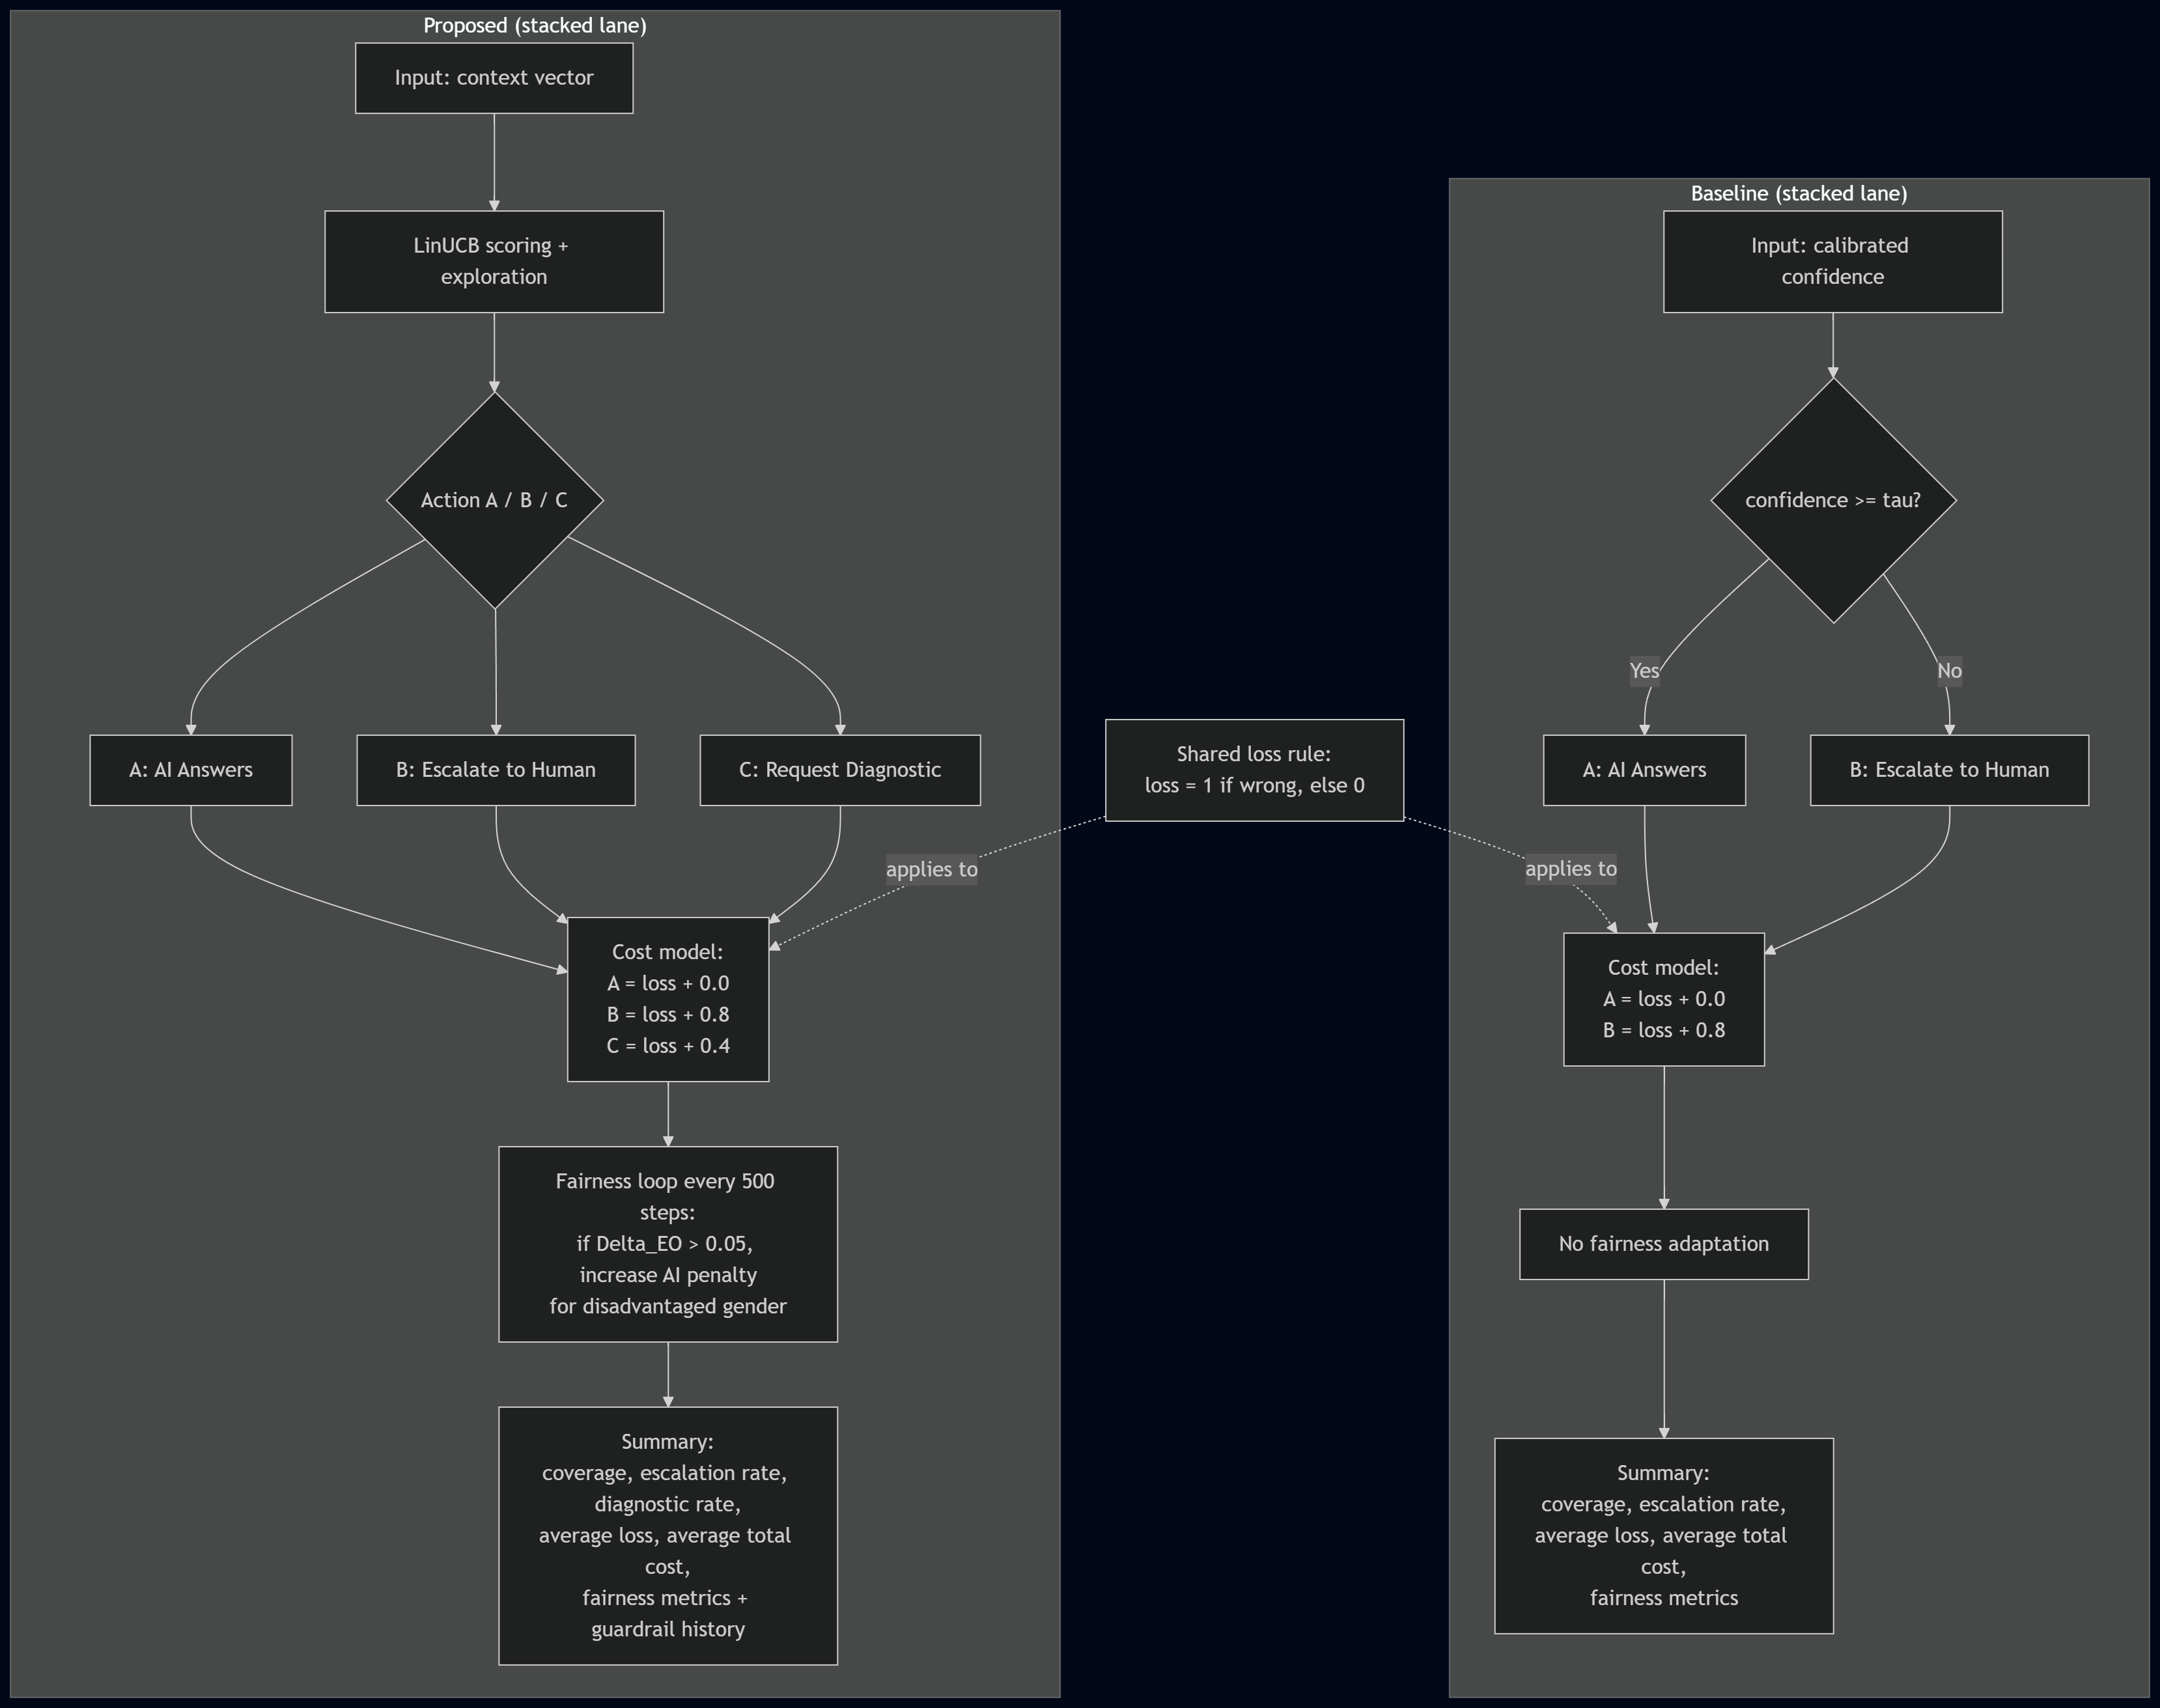
\includegraphics[width=0.94\linewidth]{../images/proposed_vs_baseline_flowchart.txt.png}
    }
  }
}
\end{center}
\vspace{-0.2cm}
\scriptsize
Baseline: confidence thresholding (\(A\) vs \(B\)). Proposed: LinUCB routing over \(A,B,C\) + fairness guardrail (\(\Delta_{EO}\)-triggered penalty updates). In all actions, the decision-maker outputs the same type of fit/not-fit judgment.
\end{frame}

% Slide 5
\begin{frame}{Results (5x Simulation Timesteps)}
\begin{columns}[T]
  \column{0.56\textwidth}
    \IfFileExists{results_reframed_proficiency_5x/risk_coverage_overall.png}
      {
\includegraphics[width=\linewidth]{results_reframed_proficiency_5x/risk_coverage_overall.png}}
      {\IfFileExists{../results_reframed_proficiency_5x/risk_coverage_overall.png}
        {
\includegraphics[width=\linewidth]{../results_reframed_proficiency_5x/risk_coverage_overall.png}}
        {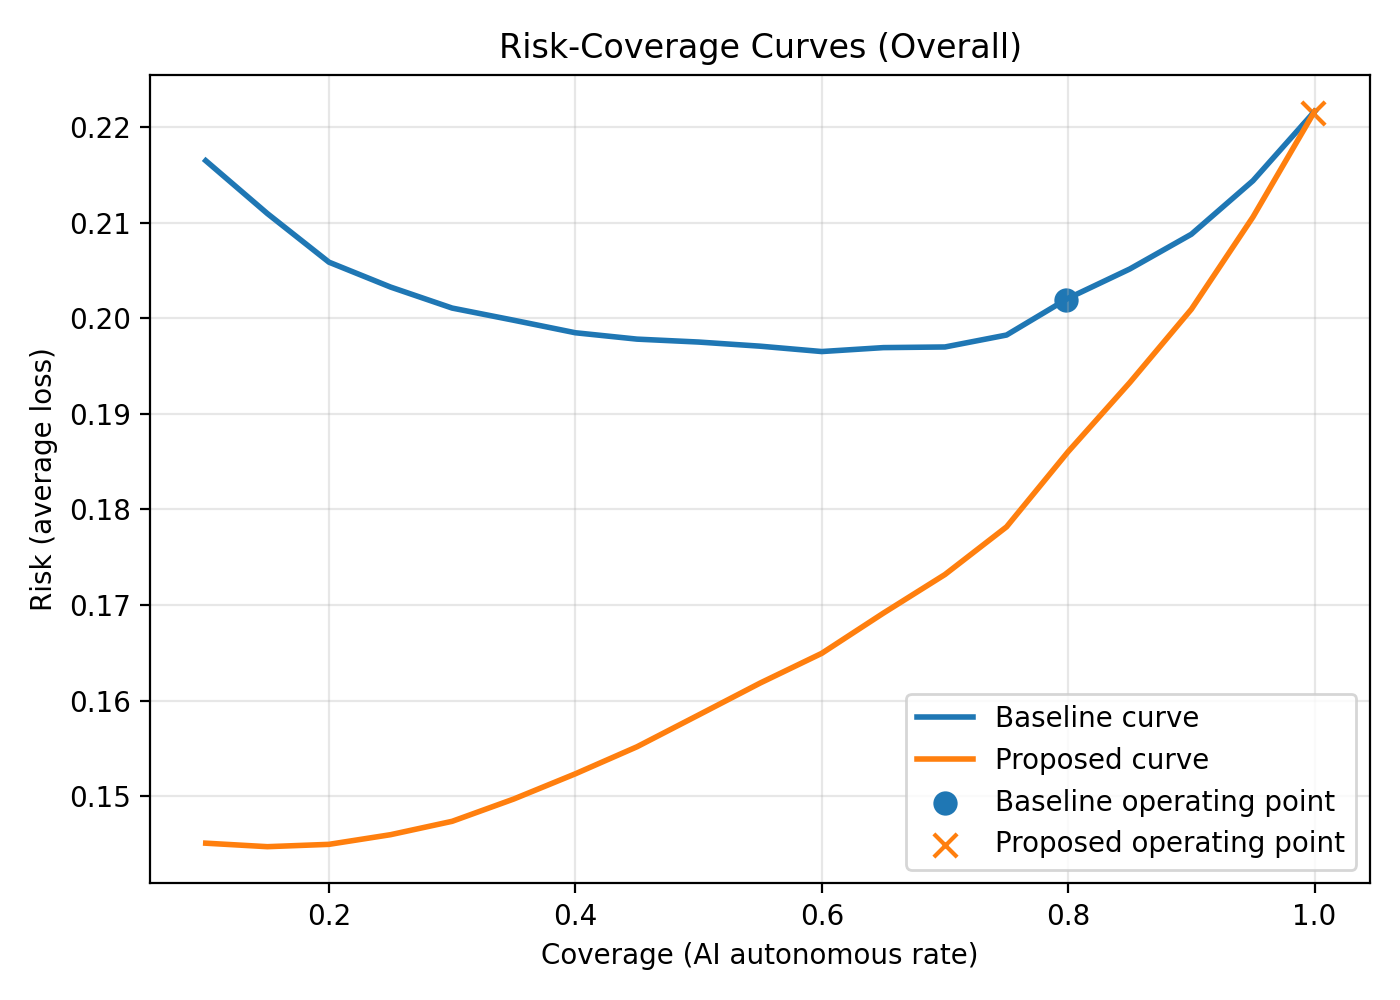
\includegraphics[width=\linewidth]{../results/risk_coverage_overall.png}}}

  \column{0.44\textwidth}
  \scriptsize
  \begin{table}
    \centering
    \begin{tabular}{lcc}
      \toprule
      Metric & Baseline & Proposed \\
      \midrule
      AI coverage & 0.798 & 0.9989 \\
      Escalation & 0.202 & 0.00009 \\
      Avg loss & 0.202 & 0.222 \\
      Avg total cost & 0.384 & 0.222 \\
      $\Delta_{\mathrm{EO}}$ (FNR) & 0.0554 & 0.0035 \\
      \bottomrule
    \end{tabular}
  \end{table}
\end{columns}

\vspace{0.15cm}
\scriptsize
\textbf{Takeaway:} On a 180k-step reframed simulation stream, proposed routing cuts average deployment cost by \(\sim\)42.1\% and reduces group disparity in proficiency-judgment FNR, while increasing task loss and still leaving high absolute FNR.
\end{frame}

\end{document}
